% Options for packages loaded elsewhere
\PassOptionsToPackage{unicode}{hyperref}
\PassOptionsToPackage{hyphens}{url}
\PassOptionsToPackage{dvipsnames,svgnames,x11names}{xcolor}
%
\documentclass[
  letterpaper,
  DIV=11,
  numbers=noendperiod]{scrartcl}

\usepackage{amsmath,amssymb}
\usepackage{iftex}
\ifPDFTeX
  \usepackage[T1]{fontenc}
  \usepackage[utf8]{inputenc}
  \usepackage{textcomp} % provide euro and other symbols
\else % if luatex or xetex
  \usepackage{unicode-math}
  \defaultfontfeatures{Scale=MatchLowercase}
  \defaultfontfeatures[\rmfamily]{Ligatures=TeX,Scale=1}
\fi
\usepackage{lmodern}
\ifPDFTeX\else  
    % xetex/luatex font selection
\fi
% Use upquote if available, for straight quotes in verbatim environments
\IfFileExists{upquote.sty}{\usepackage{upquote}}{}
\IfFileExists{microtype.sty}{% use microtype if available
  \usepackage[]{microtype}
  \UseMicrotypeSet[protrusion]{basicmath} % disable protrusion for tt fonts
}{}
\makeatletter
\@ifundefined{KOMAClassName}{% if non-KOMA class
  \IfFileExists{parskip.sty}{%
    \usepackage{parskip}
  }{% else
    \setlength{\parindent}{0pt}
    \setlength{\parskip}{6pt plus 2pt minus 1pt}}
}{% if KOMA class
  \KOMAoptions{parskip=half}}
\makeatother
\usepackage{xcolor}
\setlength{\emergencystretch}{3em} % prevent overfull lines
\setcounter{secnumdepth}{-\maxdimen} % remove section numbering
% Make \paragraph and \subparagraph free-standing
\ifx\paragraph\undefined\else
  \let\oldparagraph\paragraph
  \renewcommand{\paragraph}[1]{\oldparagraph{#1}\mbox{}}
\fi
\ifx\subparagraph\undefined\else
  \let\oldsubparagraph\subparagraph
  \renewcommand{\subparagraph}[1]{\oldsubparagraph{#1}\mbox{}}
\fi


\providecommand{\tightlist}{%
  \setlength{\itemsep}{0pt}\setlength{\parskip}{0pt}}\usepackage{longtable,booktabs,array}
\usepackage{calc} % for calculating minipage widths
% Correct order of tables after \paragraph or \subparagraph
\usepackage{etoolbox}
\makeatletter
\patchcmd\longtable{\par}{\if@noskipsec\mbox{}\fi\par}{}{}
\makeatother
% Allow footnotes in longtable head/foot
\IfFileExists{footnotehyper.sty}{\usepackage{footnotehyper}}{\usepackage{footnote}}
\makesavenoteenv{longtable}
\usepackage{graphicx}
\makeatletter
\def\maxwidth{\ifdim\Gin@nat@width>\linewidth\linewidth\else\Gin@nat@width\fi}
\def\maxheight{\ifdim\Gin@nat@height>\textheight\textheight\else\Gin@nat@height\fi}
\makeatother
% Scale images if necessary, so that they will not overflow the page
% margins by default, and it is still possible to overwrite the defaults
% using explicit options in \includegraphics[width, height, ...]{}
\setkeys{Gin}{width=\maxwidth,height=\maxheight,keepaspectratio}
% Set default figure placement to htbp
\makeatletter
\def\fps@figure{htbp}
\makeatother

\KOMAoption{captions}{tableheading}
\makeatletter
\@ifpackageloaded{caption}{}{\usepackage{caption}}
\AtBeginDocument{%
\ifdefined\contentsname
  \renewcommand*\contentsname{Table of contents}
\else
  \newcommand\contentsname{Table of contents}
\fi
\ifdefined\listfigurename
  \renewcommand*\listfigurename{List of Figures}
\else
  \newcommand\listfigurename{List of Figures}
\fi
\ifdefined\listtablename
  \renewcommand*\listtablename{List of Tables}
\else
  \newcommand\listtablename{List of Tables}
\fi
\ifdefined\figurename
  \renewcommand*\figurename{Figure}
\else
  \newcommand\figurename{Figure}
\fi
\ifdefined\tablename
  \renewcommand*\tablename{Table}
\else
  \newcommand\tablename{Table}
\fi
}
\@ifpackageloaded{float}{}{\usepackage{float}}
\floatstyle{ruled}
\@ifundefined{c@chapter}{\newfloat{codelisting}{h}{lop}}{\newfloat{codelisting}{h}{lop}[chapter]}
\floatname{codelisting}{Listing}
\newcommand*\listoflistings{\listof{codelisting}{List of Listings}}
\makeatother
\makeatletter
\makeatother
\makeatletter
\@ifpackageloaded{caption}{}{\usepackage{caption}}
\@ifpackageloaded{subcaption}{}{\usepackage{subcaption}}
\makeatother
\ifLuaTeX
  \usepackage{selnolig}  % disable illegal ligatures
\fi
\usepackage{bookmark}

\IfFileExists{xurl.sty}{\usepackage{xurl}}{} % add URL line breaks if available
\urlstyle{same} % disable monospaced font for URLs
\hypersetup{
  pdftitle={8. Funktionenscharen},
  colorlinks=true,
  linkcolor={blue},
  filecolor={Maroon},
  citecolor={Blue},
  urlcolor={Blue},
  pdfcreator={LaTeX via pandoc}}

\title{8. Funktionenscharen}
\author{}
\date{2024-03-19}

\begin{document}
\maketitle

\paragraph{Bemerkung:}\label{bemerkung}

Funktionenscharen lassen sich analog den Funktionen, auf ihre
chrakteristische Eigenschaften untersuchen. Abhängig vom Parameter
bleiben dabei:

\begin{itemize}
\tightlist
\item
  Schnittpunkte mit den Koordinatenachsen
\item
  Extrempunkte
\item
  Wendepunkte
\item
  Symmetrie
\end{itemize}

Unabhängig von t sind gemeinsame Punkte der Funktionenschar.

\paragraph{\texorpdfstring{Beispiel:
\(f_(x)=ax^4+x^3, \quad a \neq 0\)}{Beispiel: f\_(x)=ax\^{}4+x\^{}3, \textbackslash quad a \textbackslash neq 0}}\label{beispiel-f_xax4x3-quad-a-neq-0}

\begin{enumerate}
\def\labelenumi{\arabic{enumi}.}
\tightlist
\item
  Untersuchen Sie, ob alle Graphen duch den Ursprung verlaufen.
\end{enumerate}

\[
f_a(0)= 0
\] Die Lösung ist unabhänig von a und alle Graphen gehen durch den Punkt
O(0\textbar0).

\begin{enumerate}
\def\labelenumi{\arabic{enumi}.}
\setcounter{enumi}{1}
\tightlist
\item
  Bestimmen Sie \(a\) so, dass \(\int\limits_{-a}^{a} f_a(x)dx = a\)
  gilt.
\end{enumerate}

\[
\begin{aligned}
\int\limits_{-a}^{a} f_a(x)dx &= \left[\frac{1}{5}ax^5+\frac{1}{4}x^4  \right]_{-a}^a\\
&= \frac{1}{5}a\cdot a^5 + \frac{1}{4}a^4-\left( \frac{1}{5}a\cdot (-a)^5 + \frac{1}{4}(-a^)4\right)\\
&= \frac{1}{5}a^6 + \frac{1}{4}a^4 -\left(- \frac{1}{5}a^6+\frac{1}{4}a^4\right)\\
&=\frac{2}{5}a^6\\
\end{aligned}
\]

\[
\begin{aligned}
\text{Damit ergibt sich für } a>0:\\
\frac{2}{5}a^6 &=a\quad |:a\\
\frac{2}{5}a^5 &= 1\\
a^5 &=\frac{5}{2}\\
a_1 &=\sqrt[5]{\frac{5}{2}} 
\end{aligned}
\]

\[
\begin{aligned}
\text{Damit ergibt sich für }a <0:\\
\frac{2}{5}a^6 &=a\quad |:a\\
\frac{2}{5}a^5 &= 1\\
a^5 &=\frac{5}{2}\\
a_2 &=-\sqrt[5]{\frac{5}{2}} \\
\end{aligned}
\]

\begin{enumerate}
\def\labelenumi{\arabic{enumi}.}
\setcounter{enumi}{2}
\tightlist
\item
  Bestimmen Sie die Art des Extremums von \(f_a\)
\end{enumerate}

\[
\begin{aligned}
\text{1. not. Bed: } f_a'(x) &=0\\
f'_a(x) &= 4ax^3+3x^2 = 0\\
&= x^2(4ax+3) = 0\\
x_1 &= 0 \text{ und } x_2 = -\frac{3}{4a}\\
\end{aligned}
\]

\[
\begin{aligned}
\text{2. hin. Bed: } f_a''(x) &\neq 0\\
f''_a(x) &= 12ax^2+6x\\\\
\text{Für }x_1= 0\\
f''_a(0) &= 0\quad && \Rightarrow  \text{Keine Aussage möglich}\\
& && f' \text{ macht auch keinen Vorzeichenwechsel bei } x_1=0\\
& && \Rightarrow  \text{Sattelstelle}\\\\
\end{aligned}
\]

\[
\begin{aligned}
\text{Für }x_2= -\frac{3}{4a}\\
f_a''\left(-\frac{3}{4a}\right) &= \frac{108a}{16a^2}-\frac{18}{4a} = \frac{9}{4a}\\
\text{Für } a>0 \text{ gilt: lokales Minimum bei } x_2 &=-\frac{3}{4a}\\
\text{Für } a<0 \text{ gilt: lokales Maximum bei } x_2 &=-\frac{3}{4a}\\
\end{aligned}
\]

\begin{enumerate}
\def\labelenumi{\arabic{enumi}.}
\setcounter{enumi}{3}
\tightlist
\item
  Schaubild von \(f_1\), \(f_{{-1}}\), \(f_{-\frac{1}{2}}\) und \(f_2\)
\end{enumerate}

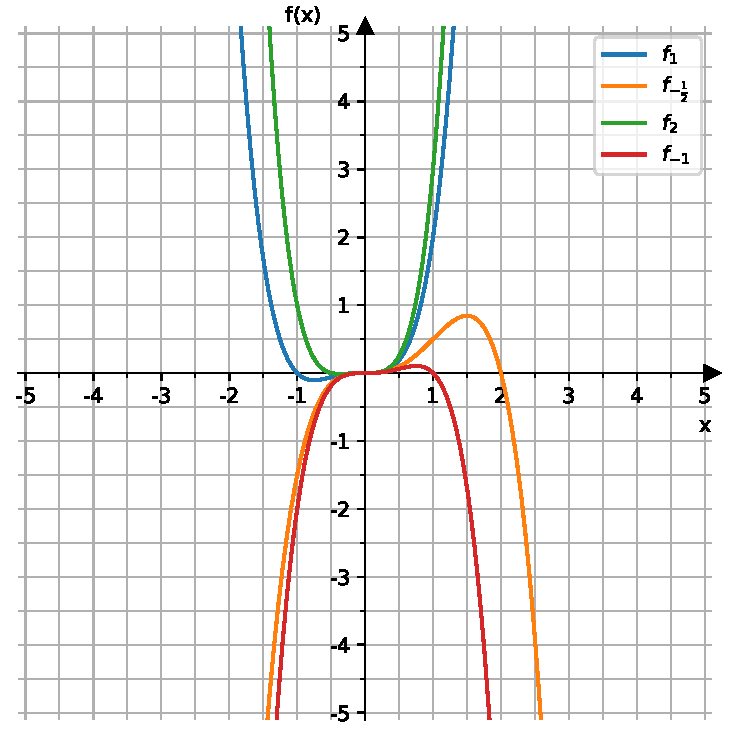
\includegraphics{8_Funktionsscharen_files/figure-pdf/cell-2-output-1.pdf}

\paragraph{Beispiel: Gemeinsame Punkte einer Funktionenschar
bestimmen}\label{beispiel-gemeinsame-punkte-einer-funktionenschar-bestimmen}

Gegeben: \(f_t(x)= (x-1)\cdot e^{-tx}, \quad t \in \mathbb{R}\)

Aufgabe: Bestimmen Sie die Koordinaten der gemeinsamen Punkte aller
Graphen \(G_{f_t}\)

Lösungsansatz 1: Verlaufen alle Graphen der Funktionenschar durch einen
Punkt, dann gilt es auch für zwei ausgewählte. Wähle zwei einfach
Vertreter, z.B. \(f_0\) und \(f_1\).

\[
\begin{aligned}
G_0 \cap G_1:&\\
x-1 &= (x-1) \cdot e^{-x} \qquad |-(x-1)\\
0 &= (x-1) \cdot e^{-x} - (x-1) \\
0 &= (x-1)\cdot (e^{-x}-1)\\
x_1 &= 1 \text{ und } x_2=0\\
f_t(1) &= 0 \text{ und } f_t(0)=-1\\
& \Rightarrow \text{Beide Werte unabhängig von }t\\ 
& \Rightarrow \text{Alle Graphen gehen durch einen gemeinsamen Punkt }t\\
& \Rightarrow P(1|0) \text { und } Q(0|-1)  
\end{aligned}
\]

Lösungsansatz 2: Löse für zwei allgemeine \(t_1\) und \(t_2\) mit
\(t_1 \neq t_2\)

\[
\begin{aligned}
G_{t_1} \cap G_{t_2}:&\\
(x-1 )e^{-t_1x} &= (x-1) \cdot e^{-t_2x} \qquad |-(x-1)e^{-t_1x}\\
0 &= (x-1) \cdot e^{-t_2x} - (x-1)e^{-t_1x} \\
0 &= (x-1)\cdot (e^{-t_2x}-e^{-t_1x})\\
x_1 &= 1 \text{ und } e^{-t_2x}-e^{-t_1x}=0\\
& e^{-t_2x}=e^{-t_1x}\\
& x_2=0\\
f_t(1) &= 0 \text{ und } f_t(0)=-1\\
& \Rightarrow \text{Beide Werte unabhängig von }t\\ 
& \Rightarrow \text{Alle Graphen gehen durch einen gemeinsamen Punkt }t\\
& \Rightarrow P(1|0) \text { und } Q(0|-1)  
\end{aligned}
\]

\paragraph{Beispiel:}\label{beispiel}

Gegeben: Funktionenschar
\(f_a(x)= x-e^{x-a}+a^2, \quad a\in \mathbb{R}\)

Aufgabe: Bestimme \(a\) so, dass der Hochpunkt der des Graphen der
Funktion \(f_a(x)\) minimal wird.

Lösung: 1. Bestimme die Hochpunkte 1. not. Bed.: \[
\begin{aligned}
f_a'(x) &=0\\
f_a'(x) &= 1-e^{x-a} = 0\\
-e^{x-a} &=-1\\
e^{x-a} &=1\\
x-a&=\ln{(1)}\\
x-a&=0\\
x&=a
\end{aligned}
\]

\begin{enumerate}
\def\labelenumi{\arabic{enumi}.}
\setcounter{enumi}{1}
\tightlist
\item
  hinr. Bed.:
\end{enumerate}

\[
\begin{aligned}
\text{2. hin. Bed: } &f_a''(x) \neq 0\\
f''_a(x) &= -e^{x-a}\\
f''_a(a) &= -e^{a-a} = -e^0 = -1\\
\Rightarrow  \text{ Hochpunkt } P \left(a|f(a) \right) &= P \left(a| a-1+a^2 \right) 
\end{aligned}
\]

\begin{enumerate}
\def\labelenumi{\arabic{enumi}.}
\setcounter{enumi}{1}
\tightlist
\item
  Die Funktion \(h(a)=a^2+a-1\) berechnet die Funktionswerte der lokalen
  Hochpunkte. Minimum bestimmen.
\end{enumerate}

\[
\begin{aligned}
\text{1. not. Bed: } &f_a'(x) =0\\
f_a'(x) &= 2a+1 = 0\\
\Leftrightarrow \quad  a &=-\frac{1}{2}\\ 
\text{2. hin. Bed: } &f_a''(x) \neq 0\\
f''_a(x) &= 2\\
f''_a\left(-\frac{1}{3}\right) &= 2 \neq 0\\
\Rightarrow  \text{ Minimum } a &=-\frac{1}{2}
\end{aligned}
\]

\begin{enumerate}
\def\labelenumi{\arabic{enumi}.}
\setcounter{enumi}{2}
\tightlist
\item
  Antwort:\\
  Für \(a=-\frac{1}{2}\) liegt der Hochpunkt \(H_a\) der Graphen
  \(G_{f_a}\) am tiefsten.
\end{enumerate}

\paragraph{Beispiel:}\label{beispiel-1}

Gegeben: Funktionsschar \(f_a(x)= x^3-ax+a, \quad a\in \mathbb{R}\)

Aufgabe: Bestimme den Flächeninhalt, den die beiden Graphen der
Funktionen \(f_{a}\) und \(f_{a-1}\) mit der y-Achse einschließen.

Lösung:

\begin{enumerate}
\def\labelenumi{\arabic{enumi}.}
\tightlist
\item
  Schnittstelle berechnen:
\end{enumerate}

\[
\begin{aligned}
f_{a}(x)&= x^3 -ax +a\\
f_{a-1}(x)&= x^3 -(a-1)x +(a-1)\\
f_a(x) &= f_{a-1}(x)\\
x^3 -ax +a &= x^3 -(a-1)x +(a-1)\qquad |-x^3\\
-ax+a &= -ax+x+a-1\\
0 &= x-1\\
1 &= x
\end{aligned}
\]

Beobachtung: Schnittstelle ist unabhängig vom Parameter \(a\).

\begin{enumerate}
\def\labelenumi{\arabic{enumi}.}
\setcounter{enumi}{1}
\tightlist
\item
  Differenzfunktion berechnen:
\end{enumerate}

\[
\begin{aligned}
f_a(x)-f_{a-1}(x)&= x^3 -ax +a - \left(x^3 -(a-1)x +(a-1)\right)\\
&=x^3 -ax +a -x^3 +(a-1)x -(a-1)\\
&=x^3-ax+a -x^3+ax-1x-a+1\\
&=-x+1
\end{aligned}
\]

Beobachtung: Differenzfunktion ist unabhängig vom Paramter \(a\).

\begin{enumerate}
\def\labelenumi{\arabic{enumi}.}
\setcounter{enumi}{2}
\tightlist
\item
  Flächeninhalt berechnen:
\end{enumerate}

\[
\begin{aligned}
A &=\int\limits_{0}^{1} f_a(x)-f_{a-1}(x)dx
&= \left[-\frac{1}{2}x^2 +x\right]_0^1 = -\frac{1}{2}1^2+1-\left(\frac{1}{2}0^2+0 \right)\\
&= \frac{1}{2}
\end{aligned}
\]

Beobachtung: Der Flächeninhalt ist unabhänging vom Paramter \(a\).

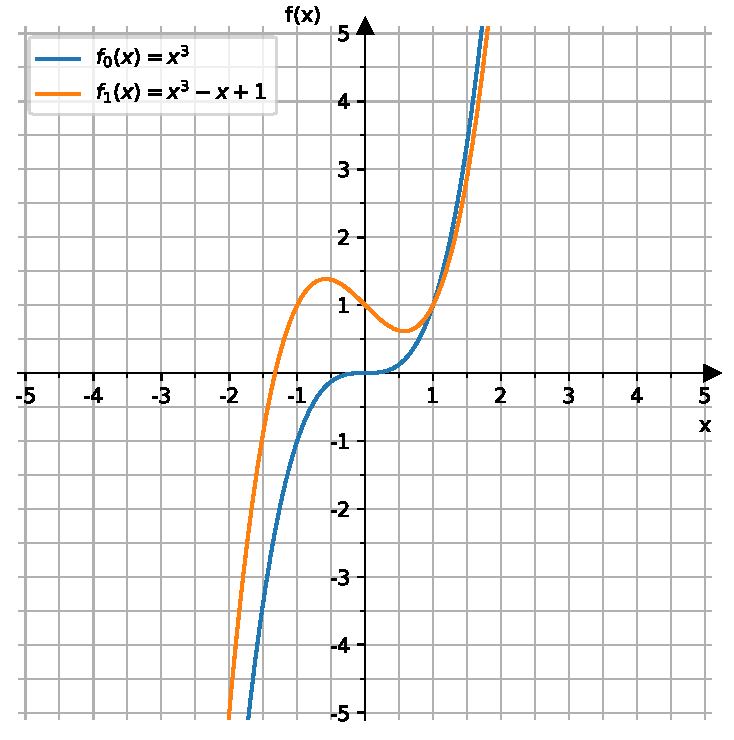
\includegraphics{8_Funktionsscharen_files/figure-pdf/cell-3-output-1.pdf}



\end{document}
